




\chapter{Glossary of terms, objects and concepts}





\section{Chapter introduction}



\section*{Human innate immune system}


\subsection*{Macrophages}


\subsection*{Neutrophils}


\subsection*{Other leukocytes}


\subsection*{Complement}


\subsection*{Cytokines}


\subsection*{Lymphatic system}



\subsection*{Bacteriophages}









\section*{Mathematical concepts}



\subsection*{Branching criticallity}


\subsubsection*{Subcritical}


\subsubsection*{Supercritical}


\subsubsection*{Critical}





\subsection*{fffff}



\subsection*{fffff}



\subsection*{fffff}




\section*{Ggggg}



\subsection*{fffff}



\subsection*{fffff}

















\begin{figure}[h!]
    \centering
    % First row of two images
    \begin{subfigure}{0.48\textwidth}
        \centering
        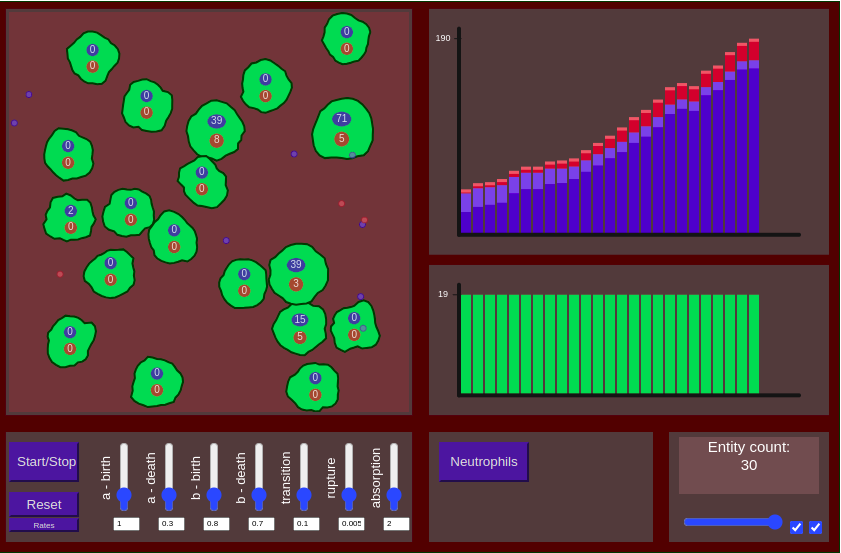
\includegraphics[width=\textwidth]{chapter2/IMG_ch2/YPwebsite/web1}
    \end{subfigure}
    \hspace{\fill}
    \begin{subfigure}{0.48\textwidth}
        \centering
        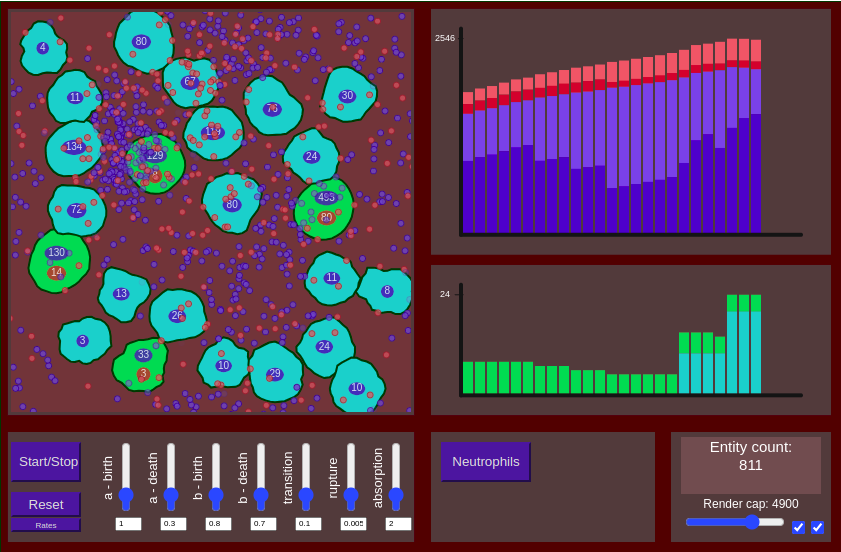
\includegraphics[width=\textwidth]{chapter2/IMG_ch2/YPwebsite/web4}
    \end{subfigure}

    \vspace{0.5em} % Small vertical space between rows

    % Second row of two images
    \begin{subfigure}{0.48\textwidth}
        \centering
        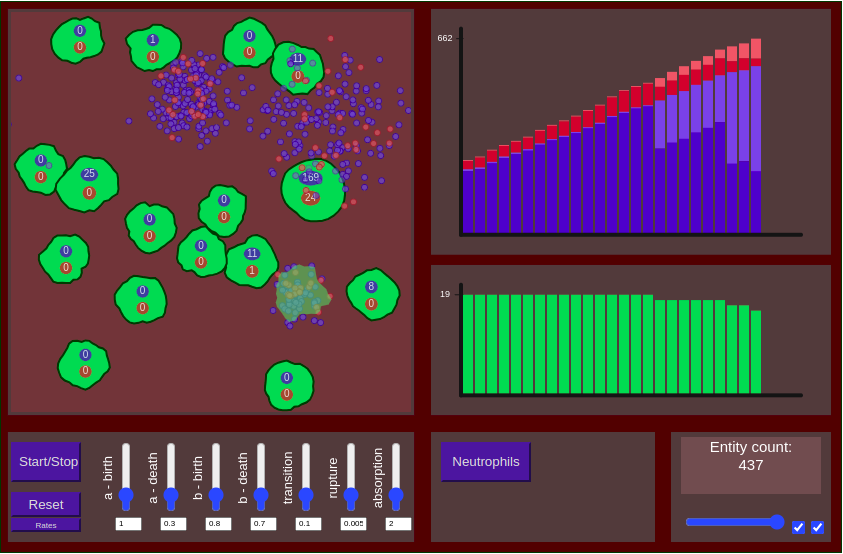
\includegraphics[width=\textwidth]{chapter2/IMG_ch2/YPwebsite/web2}
    \end{subfigure}
    \hspace{\fill}
    \begin{subfigure}{0.48\textwidth}
        \centering
        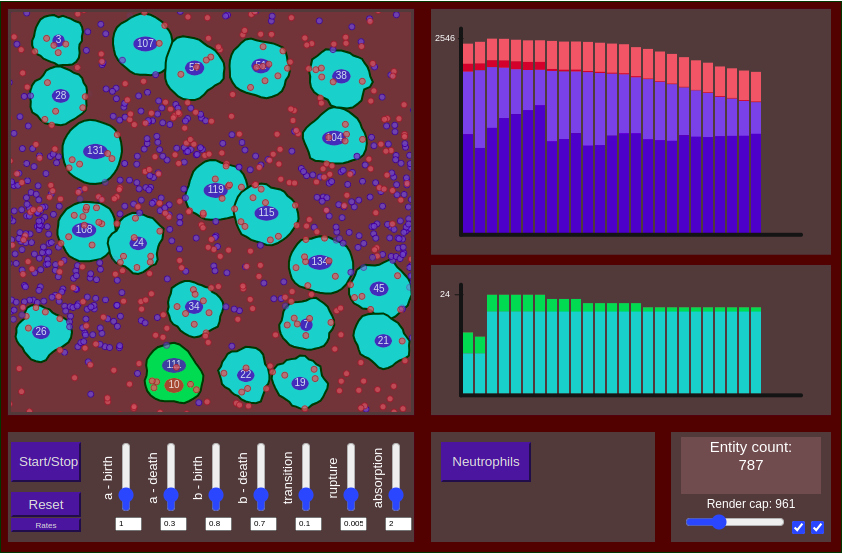
\includegraphics[width=\textwidth]{chapter2/IMG_ch2/YPwebsite/web5}
    \end{subfigure}

    \vspace{0.5em} % Small vertical space between rows

    % Third row of two images
    \begin{subfigure}{0.48\textwidth}
        \centering
        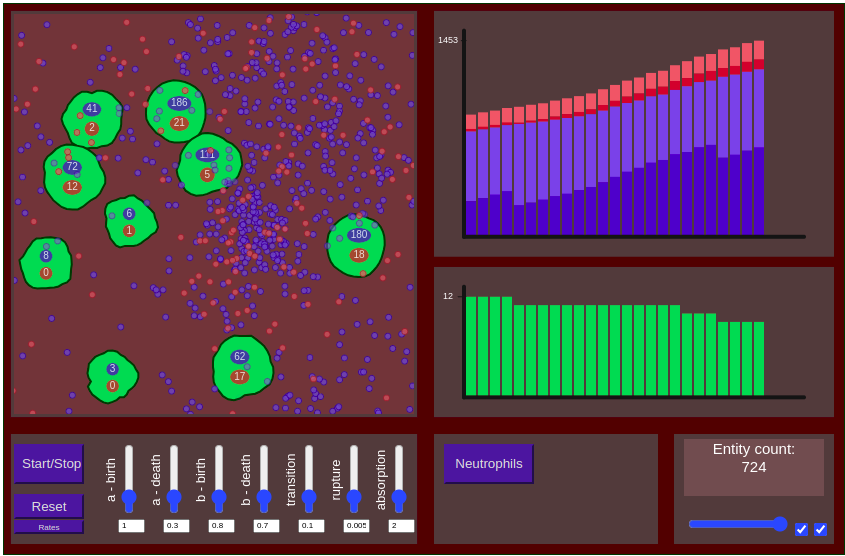
\includegraphics[width=\textwidth]{chapter2/IMG_ch2/YPwebsite/web3}
    \end{subfigure}
    \hspace{\fill}
    \begin{subfigure}{0.48\textwidth}
        \centering
        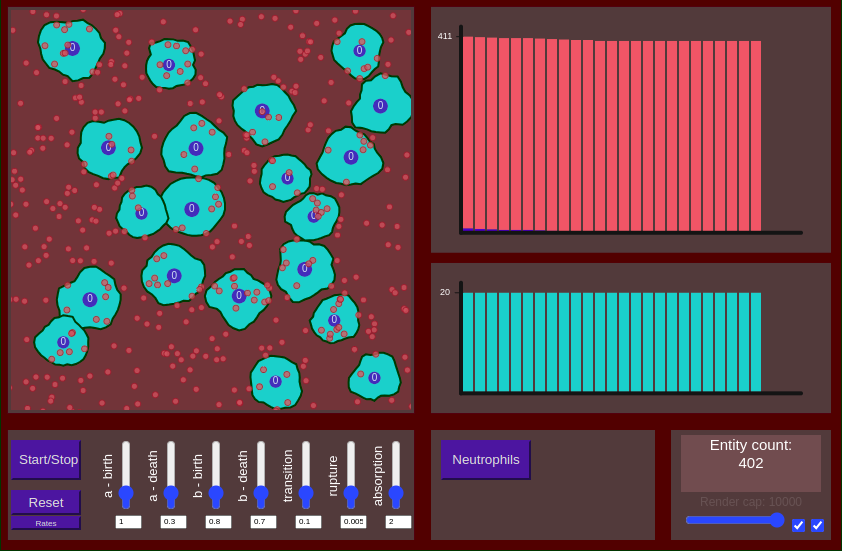
\includegraphics[width=\textwidth]{chapter2/IMG_ch2/YPwebsite/web6}
    \end{subfigure}

    % Single caption for all images
    \caption{Here we see a schematic depiction of the stages of a Y. pestis infection. At first, mostly blue phase one units replicate within green macrophages. Over time, phase one bacteria become red, changing into phase two, and the macrophages begin to burst. In this javascript (p5.js) simulation, neutrophils are recruited on demand with the push of a button. They appear suddenly and quickly absorb all phase one units in their path, killing then rapidly once engulfed. In the final slide we see only phase two bacteria floating around the extracellular matrix, unabsorbed.}
    \label{fig:two_columns_six_images}
\end{figure}






























